% This file was created with tikzplotlib v0.10.1.
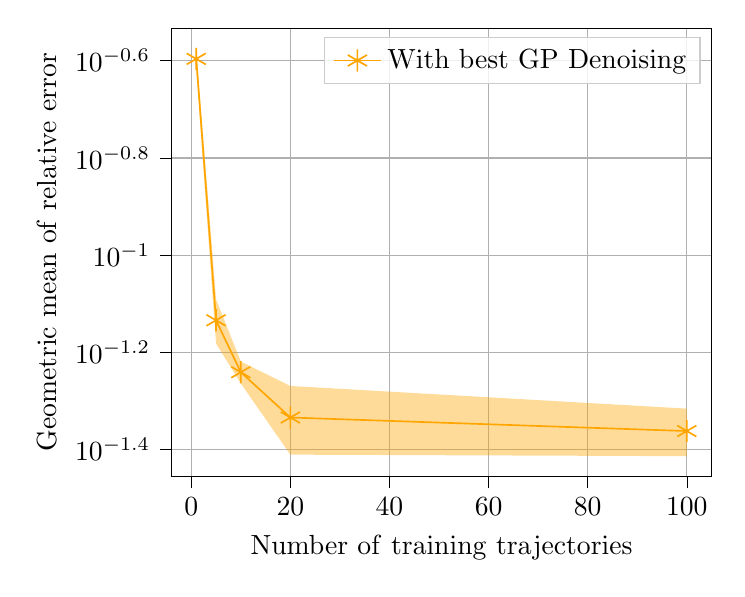
\begin{tikzpicture}

\definecolor{darkgray176}{RGB}{176,176,176}
\definecolor{lightgray204}{RGB}{204,204,204}
\definecolor{orange}{RGB}{255,165,0}

\begin{axis}[
legend cell align={left},
legend style={fill opacity=0.8, draw opacity=1, text opacity=1, draw=lightgray204},
log basis y={10},
tick align=outside,
tick pos=left,
x grid style={darkgray176},
xlabel={\(\displaystyle \mathrm{Number \ of \ training \ trajectories }\)},
xmajorgrids,
xmin=-3.95, xmax=104.95,
xtick style={color=black},
y grid style={darkgray176},
ylabel={\(\displaystyle \mathrm{Geometric \ mean \ of \ relative \ error }\)},
ymajorgrids,
ymin=0.0350511065421426, ymax=0.293015669877315,
ymode=log,
ytick style={color=black}
]
\path [fill=orange, fill opacity=0.4, semithick]
(axis cs:1,0.26605606234212)
--(axis cs:1,0.240727276762626)
--(axis cs:5,0.0658014912992053)
--(axis cs:10,0.0544682925506455)
--(axis cs:20,0.0388825584417145)
--(axis cs:100,0.0386028544998168)
--(axis cs:100,0.048349143793224)
--(axis cs:100,0.048349143793224)
--(axis cs:20,0.0538276158771443)
--(axis cs:10,0.0604246531194488)
--(axis cs:5,0.0811416705153856)
--(axis cs:1,0.26605606234212)
--cycle;

\addplot [semithick, orange, mark=asterisk, mark size=4, mark options={solid}]
table {%
1 0.253391683101654
5 0.0734715834259987
10 0.057446476072073
20 0.0463550873100758
100 0.0434760041534901
};
\addlegendentry{With best GP Denoising}
\end{axis}

\end{tikzpicture}
